% Critic network figure for the A1 poster (companion to fig_inputs_poster). Compile on its own, then:
%   \includegraphics[width=\linewidth]{images/fig_critic_poster.pdf}
% Critic inputs from learning_to_fly src/config/parameters.h (privileged observation, 31) + action (4).
\documentclass[12pt, border=4pt]{standalone}
\usepackage{tikz}
\usetikzlibrary{arrows.meta,calc,decorations.pathreplacing}
\renewcommand{\familydefault}{\sfdefault}

\definecolor{saclaydk}{RGB}{27,67,32}
\definecolor{mandarine}{RGB}{243,115,32}
\definecolor{vert}{RGB}{140,198,62}
\definecolor{bleu}{RGB}{80,144,205}
\definecolor{rouge}{RGB}{198,11,70}

\tikzset{
  cell/.style={draw=#1!70!black, fill=#1!45, line width=0.6pt},
  card/.style={draw=#1, fill=#1!10, rounded corners=4pt, line width=1.4pt},
  arr/.style={-{Stealth[length=4mm,width=3mm]}, line width=2pt},
}
\newcommand{\s}{0.36}
% \cardbox{x}{y}{title}{count}{colour}
\newcommand{\cardbox}[5]{%
  \draw[card=#5] (#1-1.15,#2-1.45) rectangle (#1+1.15,#2+1.45);
  \node[align=center, font=\large\bfseries, text=saclaydk, anchor=north] at (#1,#2+1.35) {#3};
  \node[font=\LARGE\bfseries, text=#5!60!black, anchor=south] at (#1,#2-1.4) {#4};}
% \cells{x}{y}{cols}{rows}{colour}: a grid of cells centred at (x, y)
\newcommand{\cells}[5]{%
  \foreach \i in {1,...,#3} \foreach \j in {1,...,#4}
    \draw[cell=#5] ({#1+(\i-(#3+1)/2)*\s-\s/2},{#2+(\j-(#4+1)/2)*\s-\s/2}) rectangle ++(\s,\s);}

\begin{document}
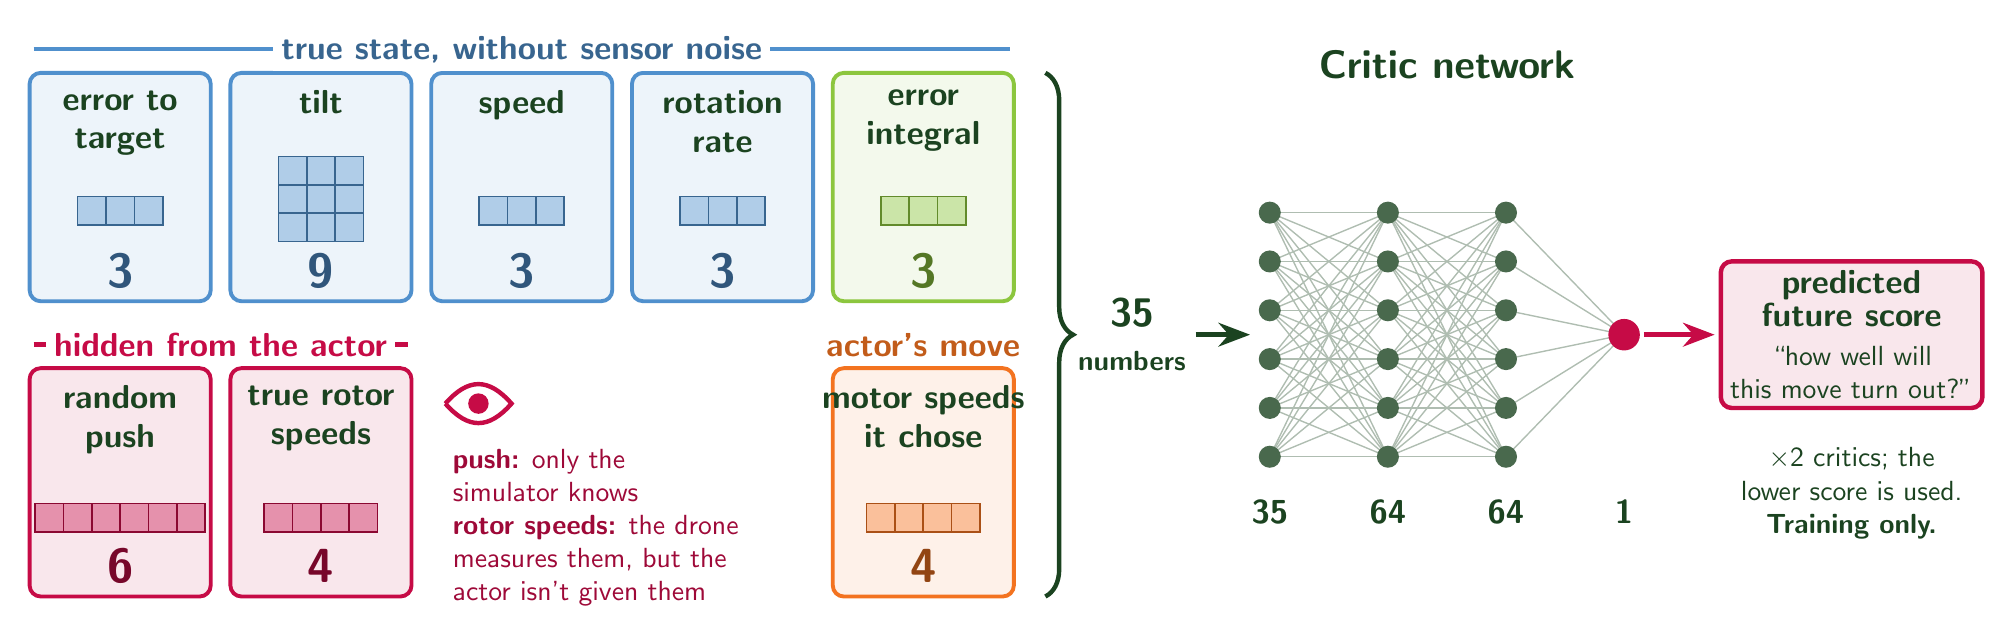
\begin{tikzpicture}
  % ---------- row 1: the true state, without sensor noise ----------
  \cardbox{0}{0}{error to\\target}{3}{bleu}       \cells{0}{-0.3}{3}{1}{bleu}
  \cardbox{2.55}{0}{tilt}{9}{bleu}                \cells{2.55}{-0.15}{3}{3}{bleu}
  \cardbox{5.1}{0}{speed}{3}{bleu}                \cells{5.1}{-0.3}{3}{1}{bleu}
  \cardbox{7.65}{0}{rotation\\rate}{3}{bleu}      \cells{7.65}{-0.3}{3}{1}{bleu}
  \cardbox{10.2}{0}{error\\integral}{3}{vert}     \cells{10.2}{-0.3}{3}{1}{vert}
  \draw[bleu, line width=1.6pt] (-1.1,1.75) -- (11.3,1.75);
  \node[font=\large\bfseries, text=bleu!70!black, fill=white, inner sep=3pt] at (5.1,1.75) {true state, without sensor noise};

  % ---------- row 2: hidden information + the actor's choice ----------
  \def\ry{-3.75}
  \cardbox{0}{\ry}{random\\push}{6}{rouge}        \cells{0}{\ry-0.45}{6}{1}{rouge}
  \cardbox{2.55}{\ry}{true rotor\\speeds}{4}{rouge} \cells{2.55}{\ry-0.45}{4}{1}{rouge}
  \draw[rouge, line width=1.6pt] (-1.1,\ry+1.75) -- (3.65,\ry+1.75);
  \node[font=\large\bfseries, text=rouge, fill=white, inner sep=3pt] at (1.275,\ry+1.75) {hidden from the actor};
  % eye + explanation
  \begin{scope}[shift={(4.55,\ry+1.0)}, line width=1.6pt, draw=rouge]
    \draw (-0.42,0) .. controls (-0.13,0.33) and (0.13,0.33) .. (0.42,0) .. controls (0.13,-0.33) and (-0.13,-0.33) .. (-0.42,0);
    \fill[rouge] (0,0) circle (0.13);
  \end{scope}
  \node[anchor=north west, align=left, font=\normalsize, text=rouge!80!black] at (4.1,\ry+0.55) {\textbf{push:} only the\\simulator knows\\\textbf{rotor speeds:} the drone\\measures them, but the\\actor isn't given them};

  \cardbox{10.2}{\ry}{motor speeds\\it chose}{4}{mandarine} \cells{10.2}{\ry-0.45}{4}{1}{mandarine}
  \draw[mandarine, line width=1.6pt] (9.1,\ry+1.75) -- (11.3,\ry+1.75);
  \node[font=\large\bfseries, text=mandarine!80!black, fill=white, inner sep=3pt] at (10.2,\ry+1.75) {actor's move};

  % ---------- bracket into the network ----------
  \draw[decorate, decoration={brace, amplitude=10pt}, line width=1.6pt, saclaydk]
    (11.75,1.45) -- (11.75,\ry-1.45);
  \node[font=\Large\bfseries, text=saclaydk, align=center] (tot) at (12.85,-1.875) {35\\[-2pt]{\normalsize numbers}};
  \draw[arr, saclaydk] (tot.east) -- (14.35,-1.875);

  % ---------- critic network ----------
  \def\ny{-1.875}
  \foreach \L/\x/\n/\sp in {0/14.6/6/0.62, 1/16.1/6/0.62, 2/17.6/6/0.62, 3/19.1/1/0.62} {
    \foreach \k in {1,...,\n} \coordinate (N\L-\k) at (\x, {\ny + (\n+1)/2*\sp - \k*\sp});
  }
  \foreach \a/\na/\b/\nb in {0/6/1/6, 1/6/2/6, 2/6/3/1}
    \foreach \i in {1,...,\na} \foreach \j in {1,...,\nb}
      \draw[saclaydk!35, line width=0.5pt] (N\a-\i) -- (N\b-\j);
  \foreach \L/\n in {0/6,1/6,2/6} \foreach \k in {1,...,\n}
    \fill[saclaydk!80] (N\L-\k) circle (0.14);
  \fill[rouge] (N3-1) circle (0.2);
  \foreach \x/\lab in {14.6/35, 16.1/64, 17.6/64, 19.1/1}
    \node[font=\large\bfseries, text=saclaydk] at (\x,\ny-2.25) {\lab};
  \node[font=\Large\bfseries, text=saclaydk] at (16.85,1.55) {Critic network};

  % ---------- output: predicted future score ----------
  \draw[arr, rouge] ($(N3-1)+(0.25,0)$) -- ++(0.9,0);
  \node[draw=rouge, fill=rouge!10, rounded corners=4pt, line width=1.6pt, align=center, anchor=west,
        font=\normalsize, text=saclaydk] (out) at (20.3,\ny)
       {{\large\bfseries predicted}\\{\large\bfseries future score}\\[2pt]``how well will\\this move turn out?''};
  \node[anchor=north, align=center, font=\normalsize, text=saclaydk] at ($(out.south)+(0,-0.35)$)
       {$\times$2 critics; the\\lower score is used.\\\textbf{Training only.}};
\end{tikzpicture}
\end{document}
